\clearpage
\section{Advanced operational amplifier applications}

	\subsection{Categories of ideal operational amplifiers}
		\begin{table}[htbp]
			\centering
			\begin{tabularx}{0.9\linewidth}{lXX} \toprule
				& Voltage output & Current output \\ \midrule
					Voltage input 
				& 
					Normal Op-Amp \newline 
					$U_a = A_D U_D$ \newline 
					\begin{center}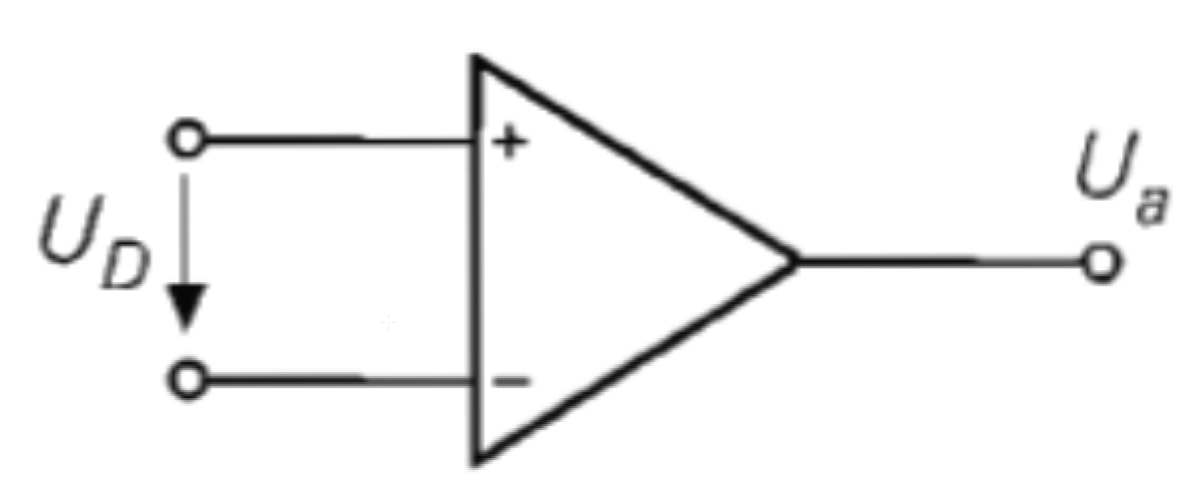
\includegraphics[width=0.25\textwidth]{images/NormalOPAMP.png}\end{center}  
				& 	Transconductance Op-Amp \newline 
					$I_a = S_D U_D$ \newline
					\begin{center}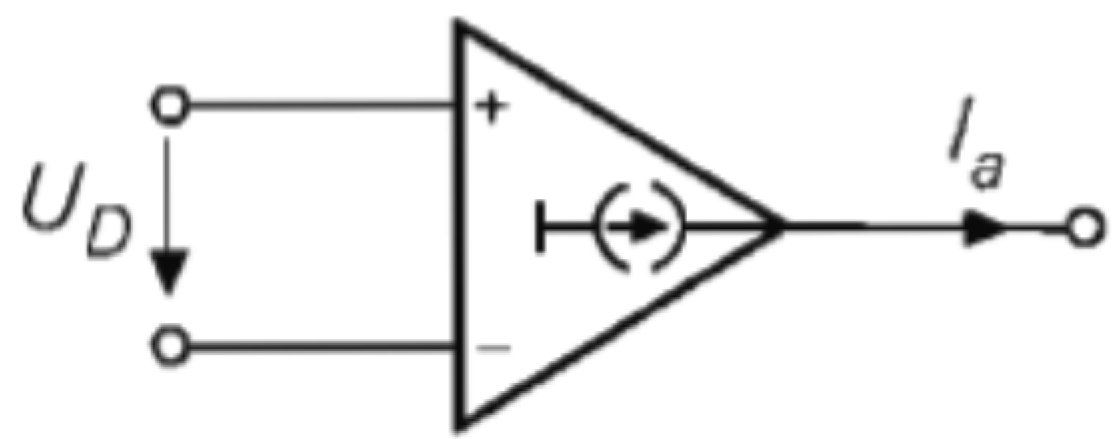
\includegraphics[width=0.25\textwidth]{images/TransconductanceOPAMP.png}\end{center}
				\\
					Current input 
				& 	Transimpedance Op-Amp \newline 
					$U_a = Z I_N$\newline
					\begin{center}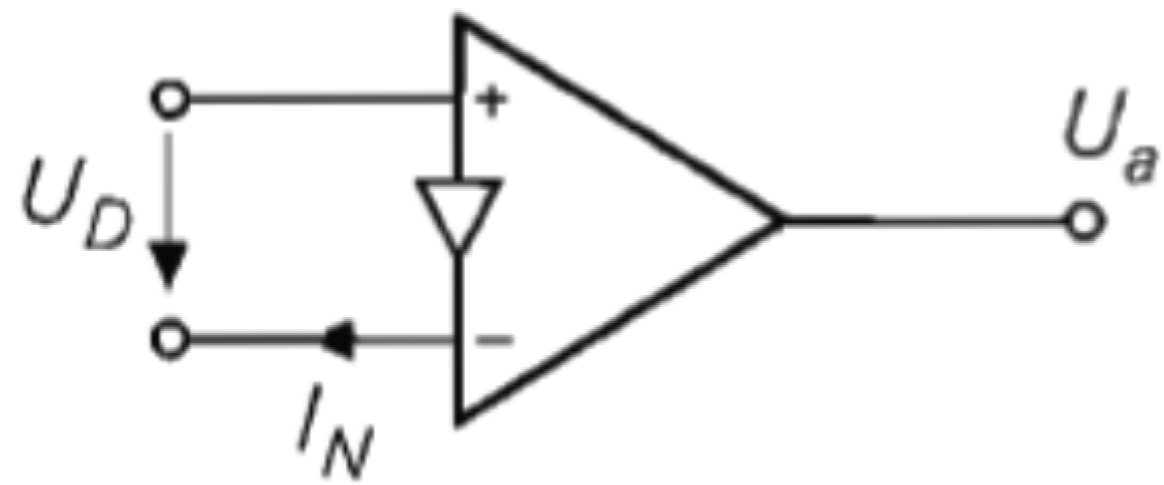
\includegraphics[width=0.25\textwidth]{images/TransimpedanceOPAMP.png}\end{center}
				 & 	Current Op-Amp \newline 
				 	$I_a = k I_N$\newline
				 	\begin{center}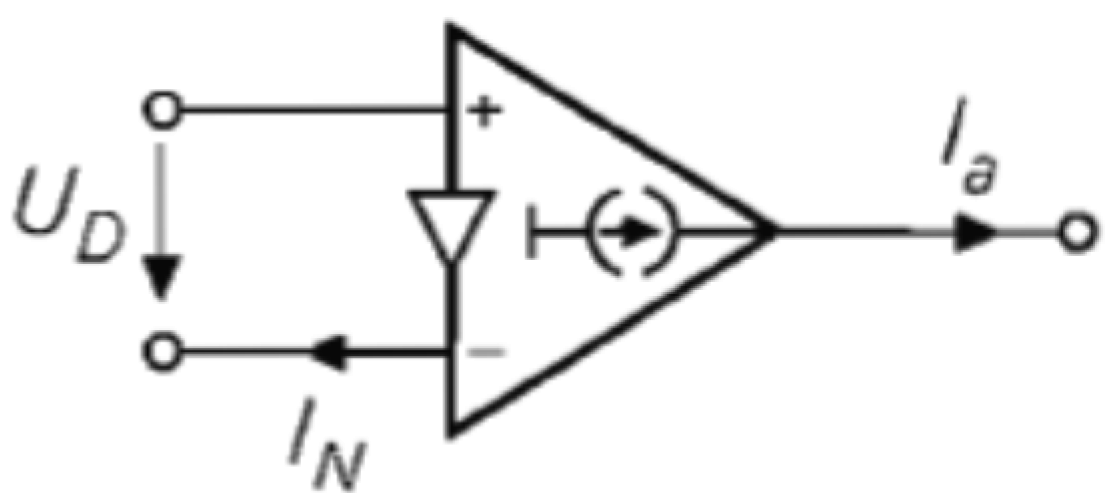
\includegraphics[width=0.25\textwidth]{images/CurrentOPAMP.png}\end{center} \\ \bottomrule
			\end{tabularx}
		\end{table}
	
	
	\subsection{Control loop block diagram}
		\begin{figure}[h]
			\centering
			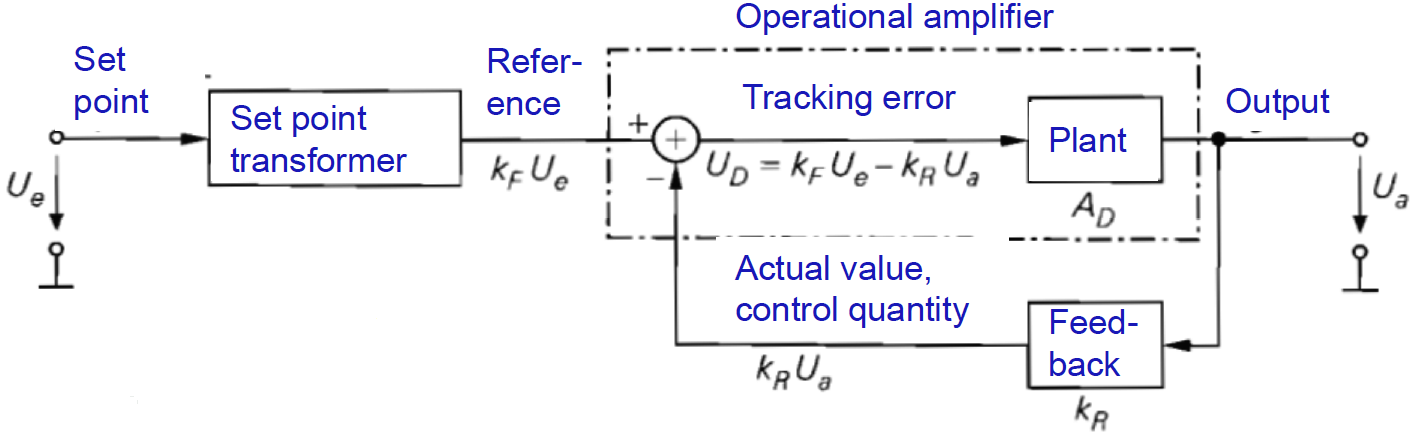
\includegraphics[width=0.75\textwidth]{images/ControlLoopDiagram.png}
			\caption{Control Loop Block Diagram}
			\label{Fig:ControlLoopDiagram}
		\end{figure}
	
		\begin{table}[htbp]
			\centering
			\begin{tabular}{llll}
				Open-loop gain & $A_D$ & Closed-loop gain & $A$\\
				Feedback loop gain & $g$ & Feedback factor & $k_R$\\
			\end{tabular}
		\end{table}
		
		\begin{align}
			U_D &= k_F U_e - k_R U_a \\
			A &= \frac{U_a}{U_e} = \frac{k_F A_D}{1 + k_R A_D} \cong \frac{k_F}{k_R}
		\end{align}
	
	\subsubsection{Non-inverting amplifier}
		\begin{figure}[h]
			\centering
			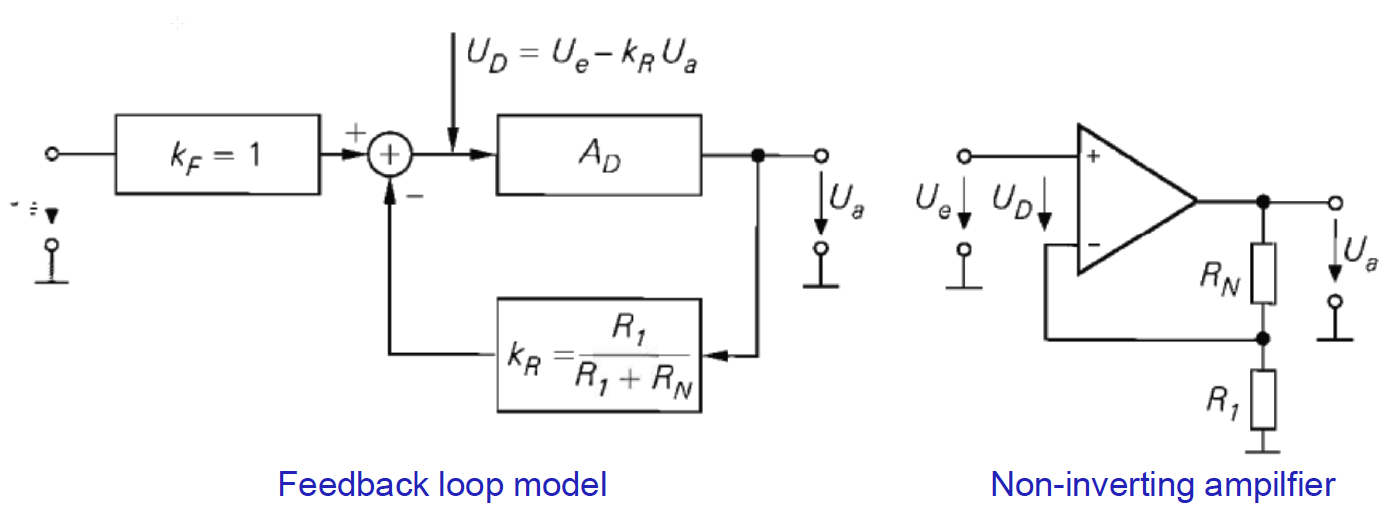
\includegraphics[width=0.75\textwidth]{images/ControlLoopNonInvertingDiagram.png}
			\caption{Control Loop Block Diagram of non-inverting amp}
			\label{Fig:ControlLoopNonInvertingDiagram}
		\end{figure}
		\begin{align}
			k_F &= 1 \\
			k_R &= \frac{R_1}{R_1 + R_N} \\
			A &= \frac{U_a}{U_e} = \frac{A_D}{1 + k_R A_D} \cong \frac{1}{k_R} = 1 + \frac{R_N}{R_1}
		\end{align}
		\begin{itemize}
			\setlength{\itemsep}{-5pt}
			\item Simpflication only valid if loop gain $g = k_R A_D$ is very high. 
			\item Distinguish between:
			\item[] Open loop gain \textbf{$A_D$}
			\item[] Closed loop gain \textbf{$A$}
			\item[] Feedback loop gain \textbf{$g$}
			\item[] Feedback factor \textbf{$k_R$ }
		\end{itemize}
	\subsubsection{Inverting amplifier}
		\begin{figure}[h]
			\centering
			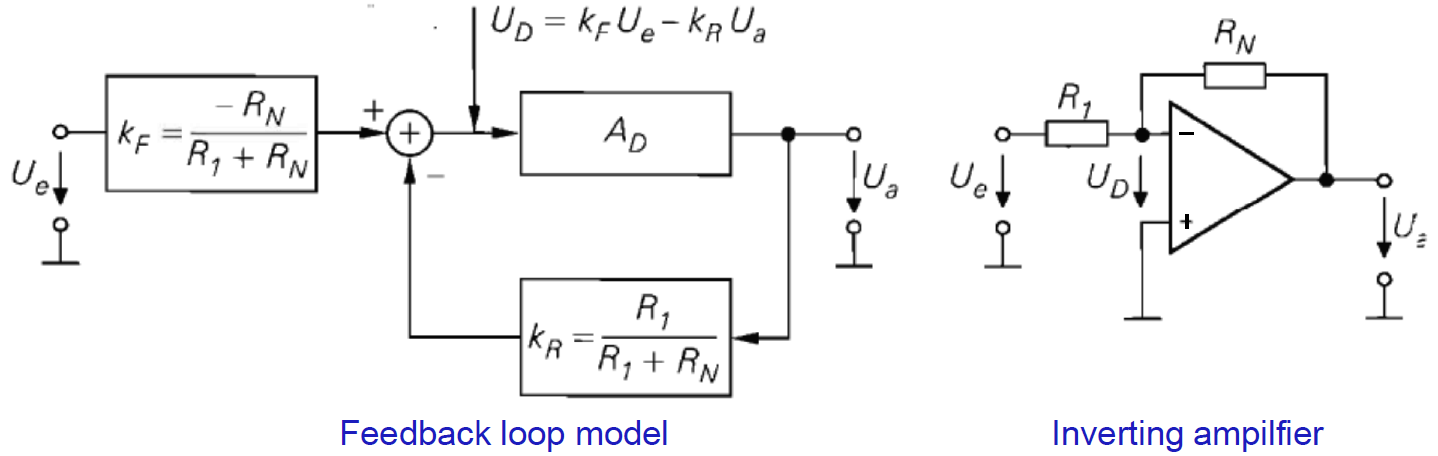
\includegraphics[width=0.75\textwidth]{images/ControlLoopInvertingDiagram.png}
			\caption{Control Loop Block Diagram of inverting amp}
			\label{Fig:ControlLoopInvertingDiagram}
		\end{figure}
		\begin{align}
			k_F &= -\frac{R_N}{R_1 + R_N} \\
			k_R &= \frac{R_1}{R_1 + R_N} \\
			A &= \frac{U_a}{U_e} \cong -\frac{R_N}{R_1}
		\end{align}
	
	\newpage
	\subsubsection{Differential amplifier}
			\begin{figure}[h]
				\centering
				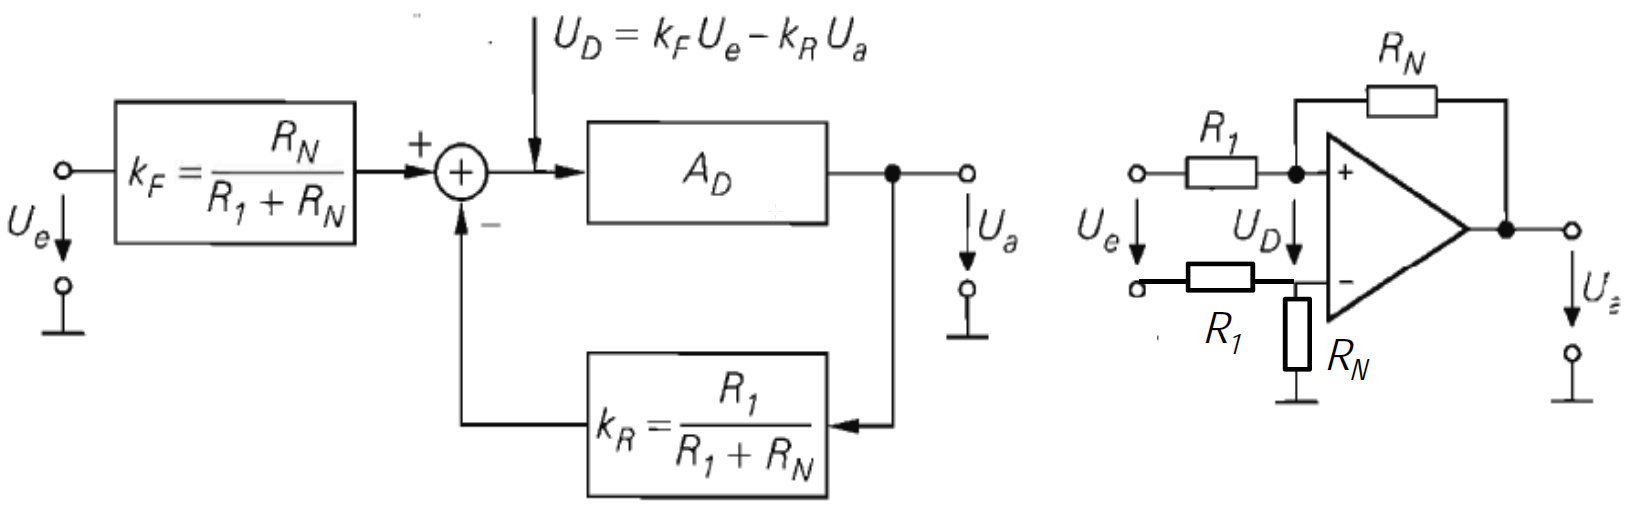
\includegraphics[width=0.75\textwidth]{images/ControlLoopDiffDiagram.png}
				\caption{Control Loop Block Diagram of differential amp}
				\label{Fig:ControlLoopDiffDiagram}
			\end{figure}
		    \begin{align}
		    	k_F &= ...\\
		    	k_R &= \\
		    	A &=  \\
		    	U_a &= \frac{R_N}{R_1}\left(U_{e+}-U_{e-}\right)
		    \end{align}
	
	\subsection{Op-Amp building blocks}
		\subsubsection{Differential pair}
			Large signal analysis: \\
			\begin{table}[h!]
				\centering
				\begin{tabular}{m{0.45\textwidth} m{0.35\textwidth} }
					
					\begin{center}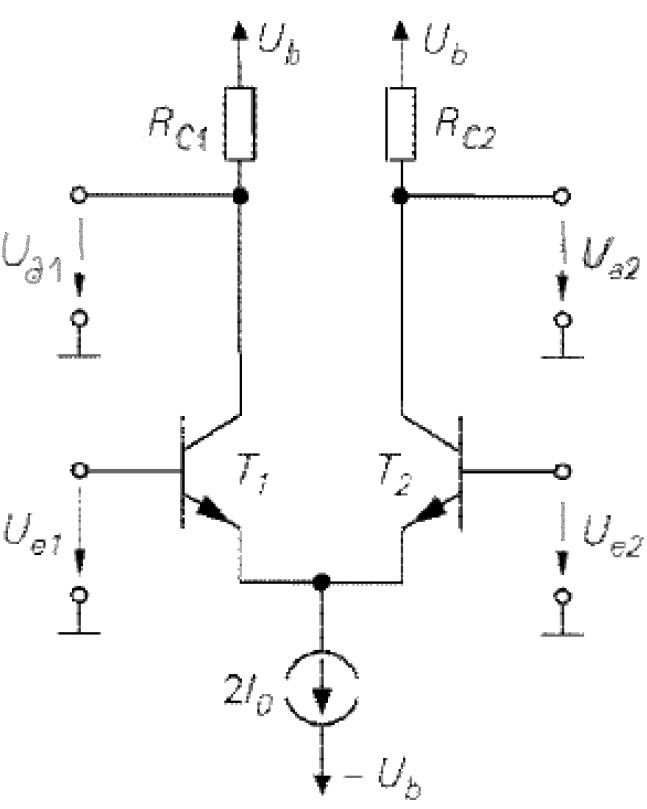
\includegraphics[width=0.25\textwidth]{images/Differenzverstaerker.png}\end{center} 
				&
							
					$I_{C1} = I_0 + \Delta I = I_0 \left( 1 + \tanh\frac{U_D}{2 U_T} \right)$\newline
					$I_{C2} = I_0 - \Delta I = I_0 \left( 1 - \tanh\frac{U_D}{2 U_T} \right)$

				\\
			
				\end{tabular}
			\end{table}			
		
		
			Small signal analysis, for $R_E >> r_S$ : \\
			\begin{table}[h!]
				\centering
				\begin{tabular}{m{0.45\textwidth} m{0.35\textwidth} }
					
					\begin{center}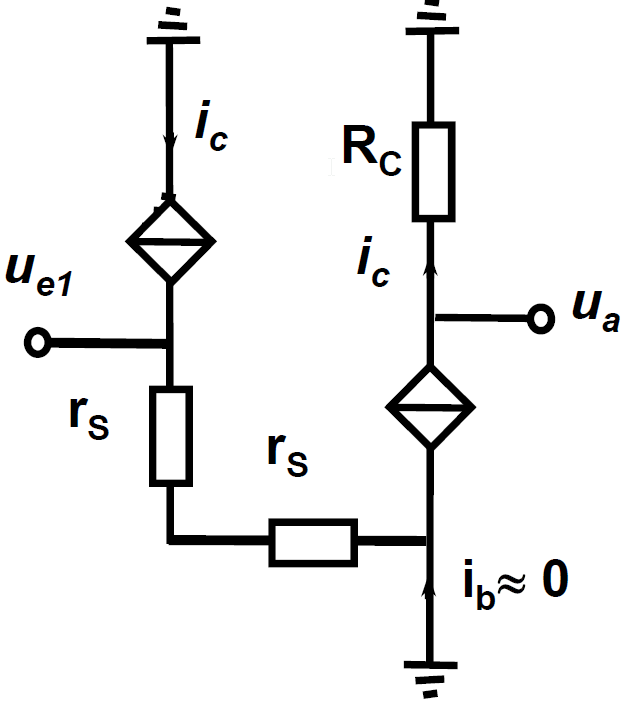
\includegraphics[width=0.25\textwidth]{images/Differenzverstaerker2.png}\end{center} 
				&
							
					$\frac{u_a}{u_{e1}} = \frac{R_C}{2 r_S}$\newline
					$\frac{u_a}{u_{e2}} = -\frac{R_C}{2 r_S}$

				\\
			
				\end{tabular}
			\end{table}				

	
		\subsubsection{Current mirror}
			\begin{multicols}{2}
				\begin{center}
					\begin{circuitikz}[scale=0.8,transform shape]
	\draw 
		(0,0) node[anchor=east] {$U_b$} to[R=$R_V$] (2,0)
		(3,-1) node[npn,xscale=-1] (t1) {}
		(6,-1) node[npn] (t2) {}
		(2,0) -| (t1.C)
		(2,0) -| (t1.B)
		(t1.B) -- (t2.B)
		(7,0) -| (t2.C)
		(t1.E) to[R=$R_1$] (3,-3.5) to (3,-4) node[rground] {}
		(t2.E) to[R=$R_2$] (6,-3.5) to (6,-4) node[rground] {}
	;		
\end{circuitikz}
				\end{center}
				\vfill
				\columnbreak
				The emitter current $I_e$ of $T1$ is
				\begin{align}
					I_e = \frac{U_b - U_{BE1}}{R_V + R_1}
				\end{align}
				The output resistance is
				\begin{align}
					r_a = \left.\frac{u_a}{i_a}\right|_{i_e=0} \cong r_{CE2} \left( 1 + \frac{\beta R_2}{R_1 + R_2 + r_{BE2}} \right)
				\end{align}
			\end{multicols}
			
			The current mirror is used as current source and active load in differential pairs to replace the resistors. 
			It allows to achieve high gains at low supply voltage.
		
		\newpage
		\subsubsection{Cascode circuit}
			Current mirror with cascode circuit increases the output resistance. 
			\begin{multicols}{2}
				\begin{center}
					\begin{circuitikz}[scale=0.8,transform shape]
	\draw 
		(0,0) node[npn] (t2) {$T_2$}
		(0,-2) node[npn] (t1) {$T_1$}
		(0,3) node[anchor=south] {$U_b$} to[R=$R_C$] (t2.C) (0,1) -- (1.5,1) node[anchor=west] {$U_a$}
		(t2.E) -- (t1.C)
		(t1.E) -- (0,-3) node[rground] {}
		(-2,-2) node[anchor=east] {$U_e$} -- (t1.B)
		(-2,0) node[anchor=east] {$U_0$} -- (t2.B)
	;
\end{circuitikz}
				\end{center}
				\vfill
				\columnbreak
				$T_1$ is in common emitter, $T_2$ in common base.
				\begin{align}
					A &= \frac{u_a}{u_e} = A_E \frac{r_{e,B}}{r_{a,E} + r_{e,B}} A_B \nonumber \\
					 &= -\frac{r_{CE1}}{r_{S1}} \frac{r_{S2}}{r_{CE1}+r_{s2}} \frac{R_C}{r_{s2}} \cong \frac{R_C}{r_{s1}}
				\end{align}
				While the gain is identical, the output resistance is higher and the emitter stage has only gain $-1$ and thus only has a Miller capacitance of
				\begin{align}
					C_e = C_M \left( 1 + |A_{E,op}| \right) \cong 2 C_M
				\end{align}
			\end{multicols}
			
			Figure below shows a comparison about the improvements obtained by using active load and cascode circuits with regard to the static gain and the bandwidth. \\
			$\rightarrow$ More gain \& more bandwidth!
			\begin{figure}[h]
				\centering
				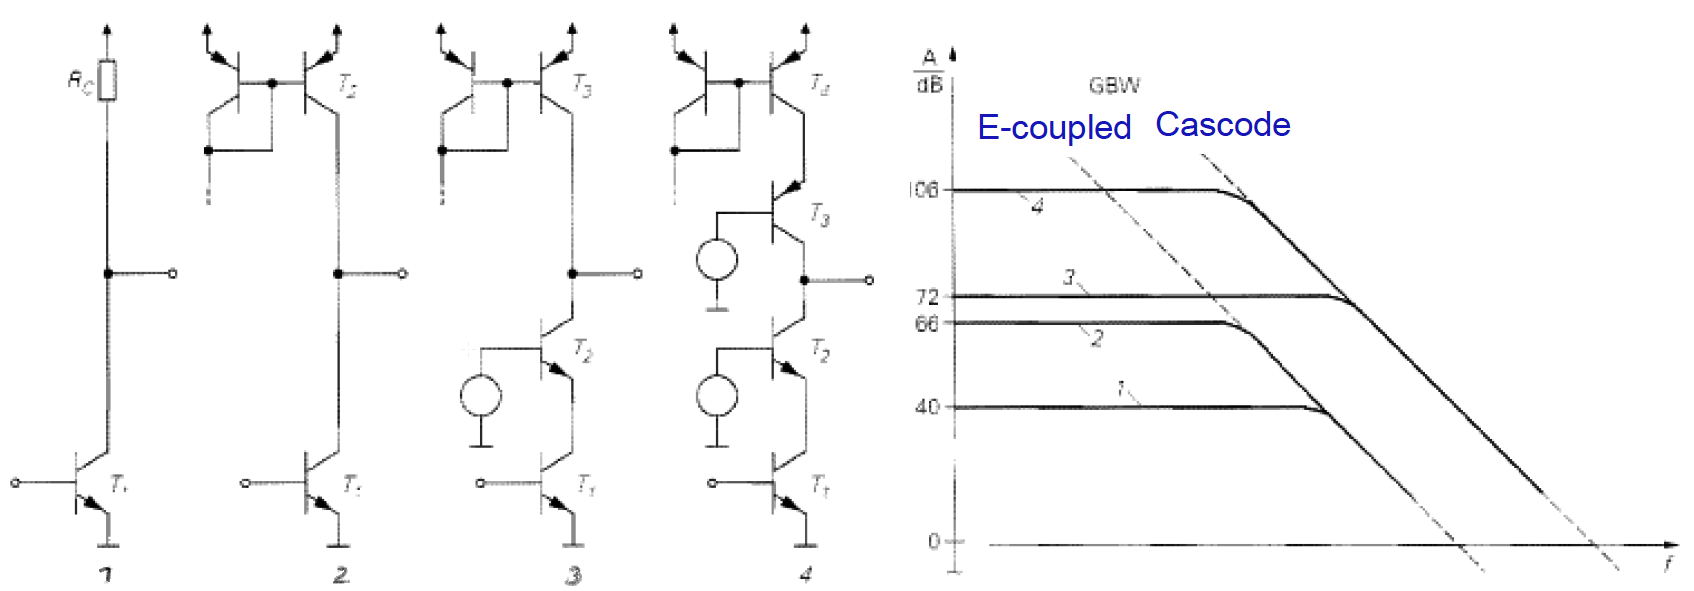
\includegraphics[width=0.75\textwidth]{images/Comparison.png}
				\caption{}
				\label{Fig:Comparison}
			\end{figure}
			\\
			See also Slides 14 to 16 in OPAMP1 for further info about the cascode circuit. 

	\subsubsection{Level Shifting}
		Level shifting can be accomplished by either using Z-Diode or complementary transistors or very fancy circuit with current mirror. 
		See pages 21 to 24 in OPAMP1 for further info. 
		
	\subsubsection{Darlington Transistor}
		Advantages: \\
		Strong increase of current gain and input resistance as compared to single transistor. 
		See pages 27 in OPAMP1 for schematic. 
		
	\subsubsection{Supply Voltages}
		Rail-To-Rail OPAMP do not have a dropout voltage, meaning their signals can reach the maximum and the minimum of the supply voltage. Normal OPAMPs do have a dropout voltage. \\
		$\rightarrow$ Single Supply Amplifier LM324 see slide 31 of OPAMP1! \\
		$\rightarrow$ Single Supply CMOS AMP slide 33 of OPAMP1\\
		$\rightarrow$ Rail-To-Rail I/O OPAMP slide 35 of OPAMP1